\chapter{Implementation}\label{ch:5}
\subsection{Tech Stack}

\begin{figure}[h]
    \centering
    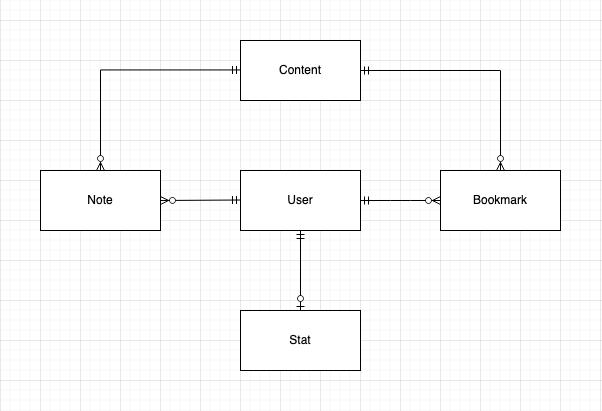
\includegraphics[scale=0.5]{figures/erd.png}
    \caption{Entity Relationship Diagram}
    \label{fig:gp}
\end{figure}

\pagebreak
Frontend: React.js, Tailwind.css, Next.js \\
Backend: Next.js \\
Database: PostgreSQL \\


\subsection{Wireframes}

\begin{figure}[h]
    \centering
    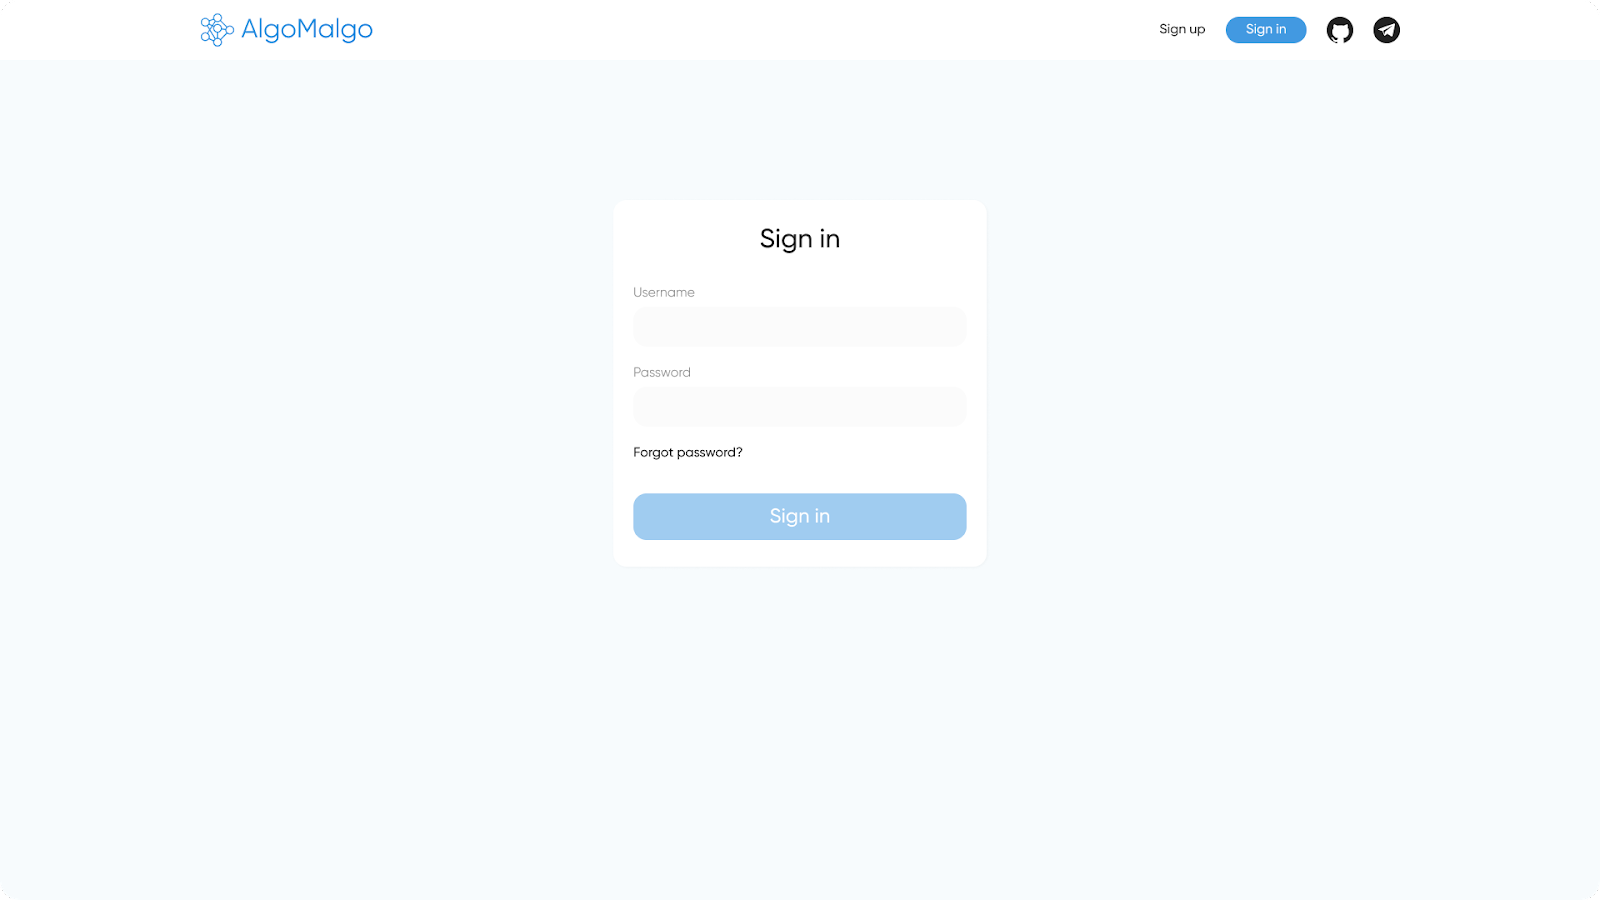
\includegraphics[scale=0.3]{figures/signin.png}
    \caption{Sign In}
    \label{fig:gp}
\end{figure}

\pagebreak

\begin{figure}[h]
    \centering
    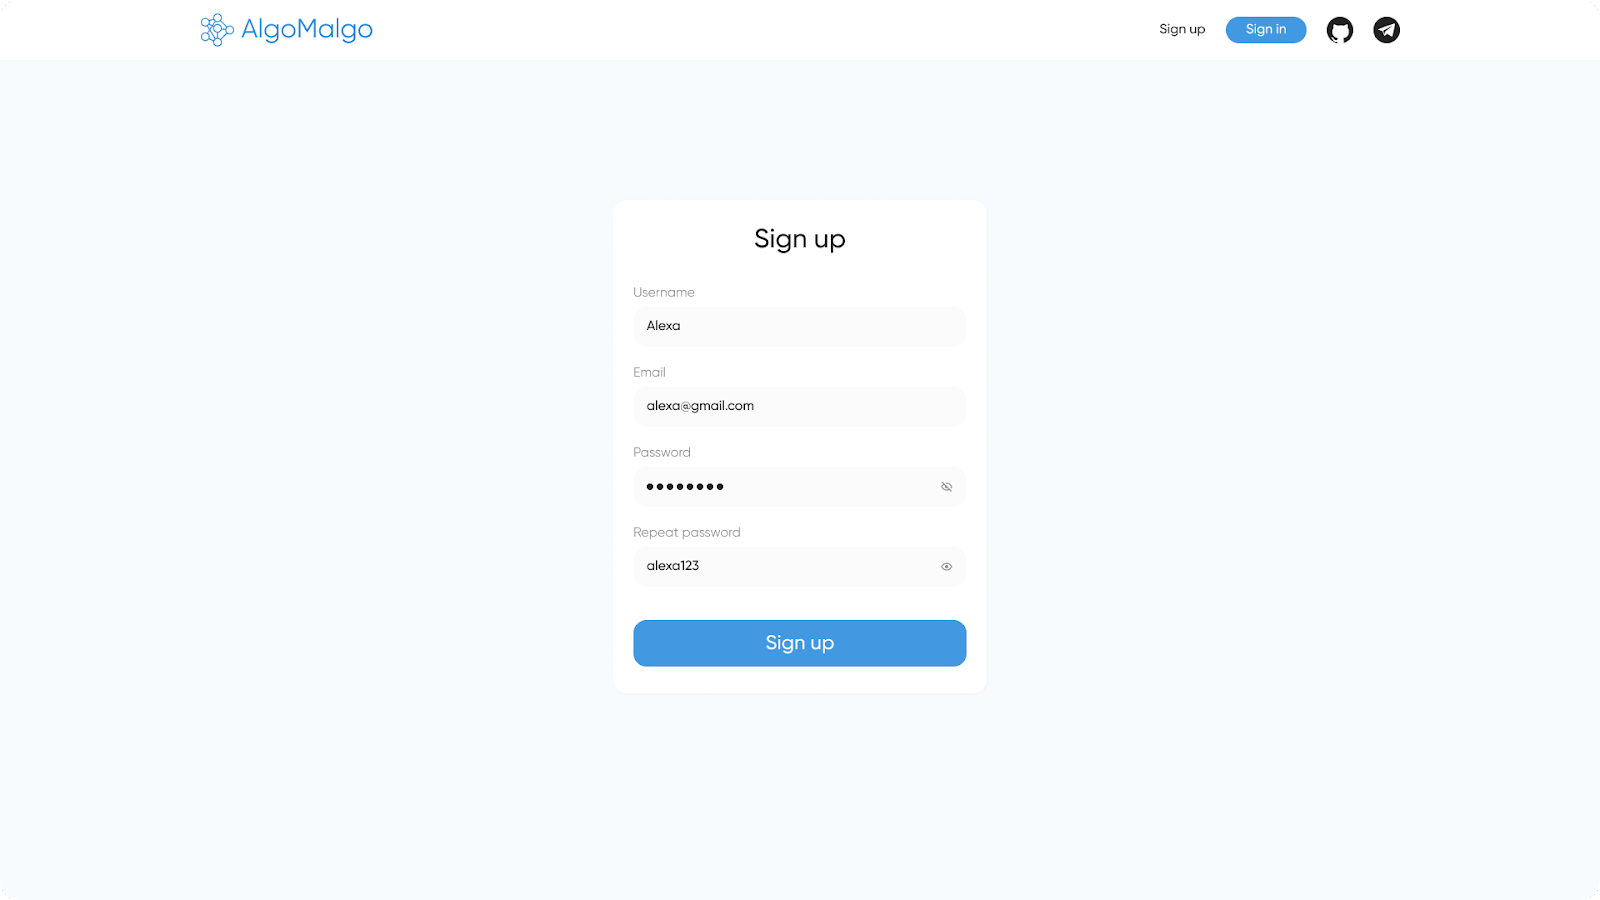
\includegraphics[scale=0.3]{figures/registration.png}
    \caption{Registration}
    \label{fig:gp}
\end{figure}

\pagebreak

\begin{figure}[h]
    \centering
    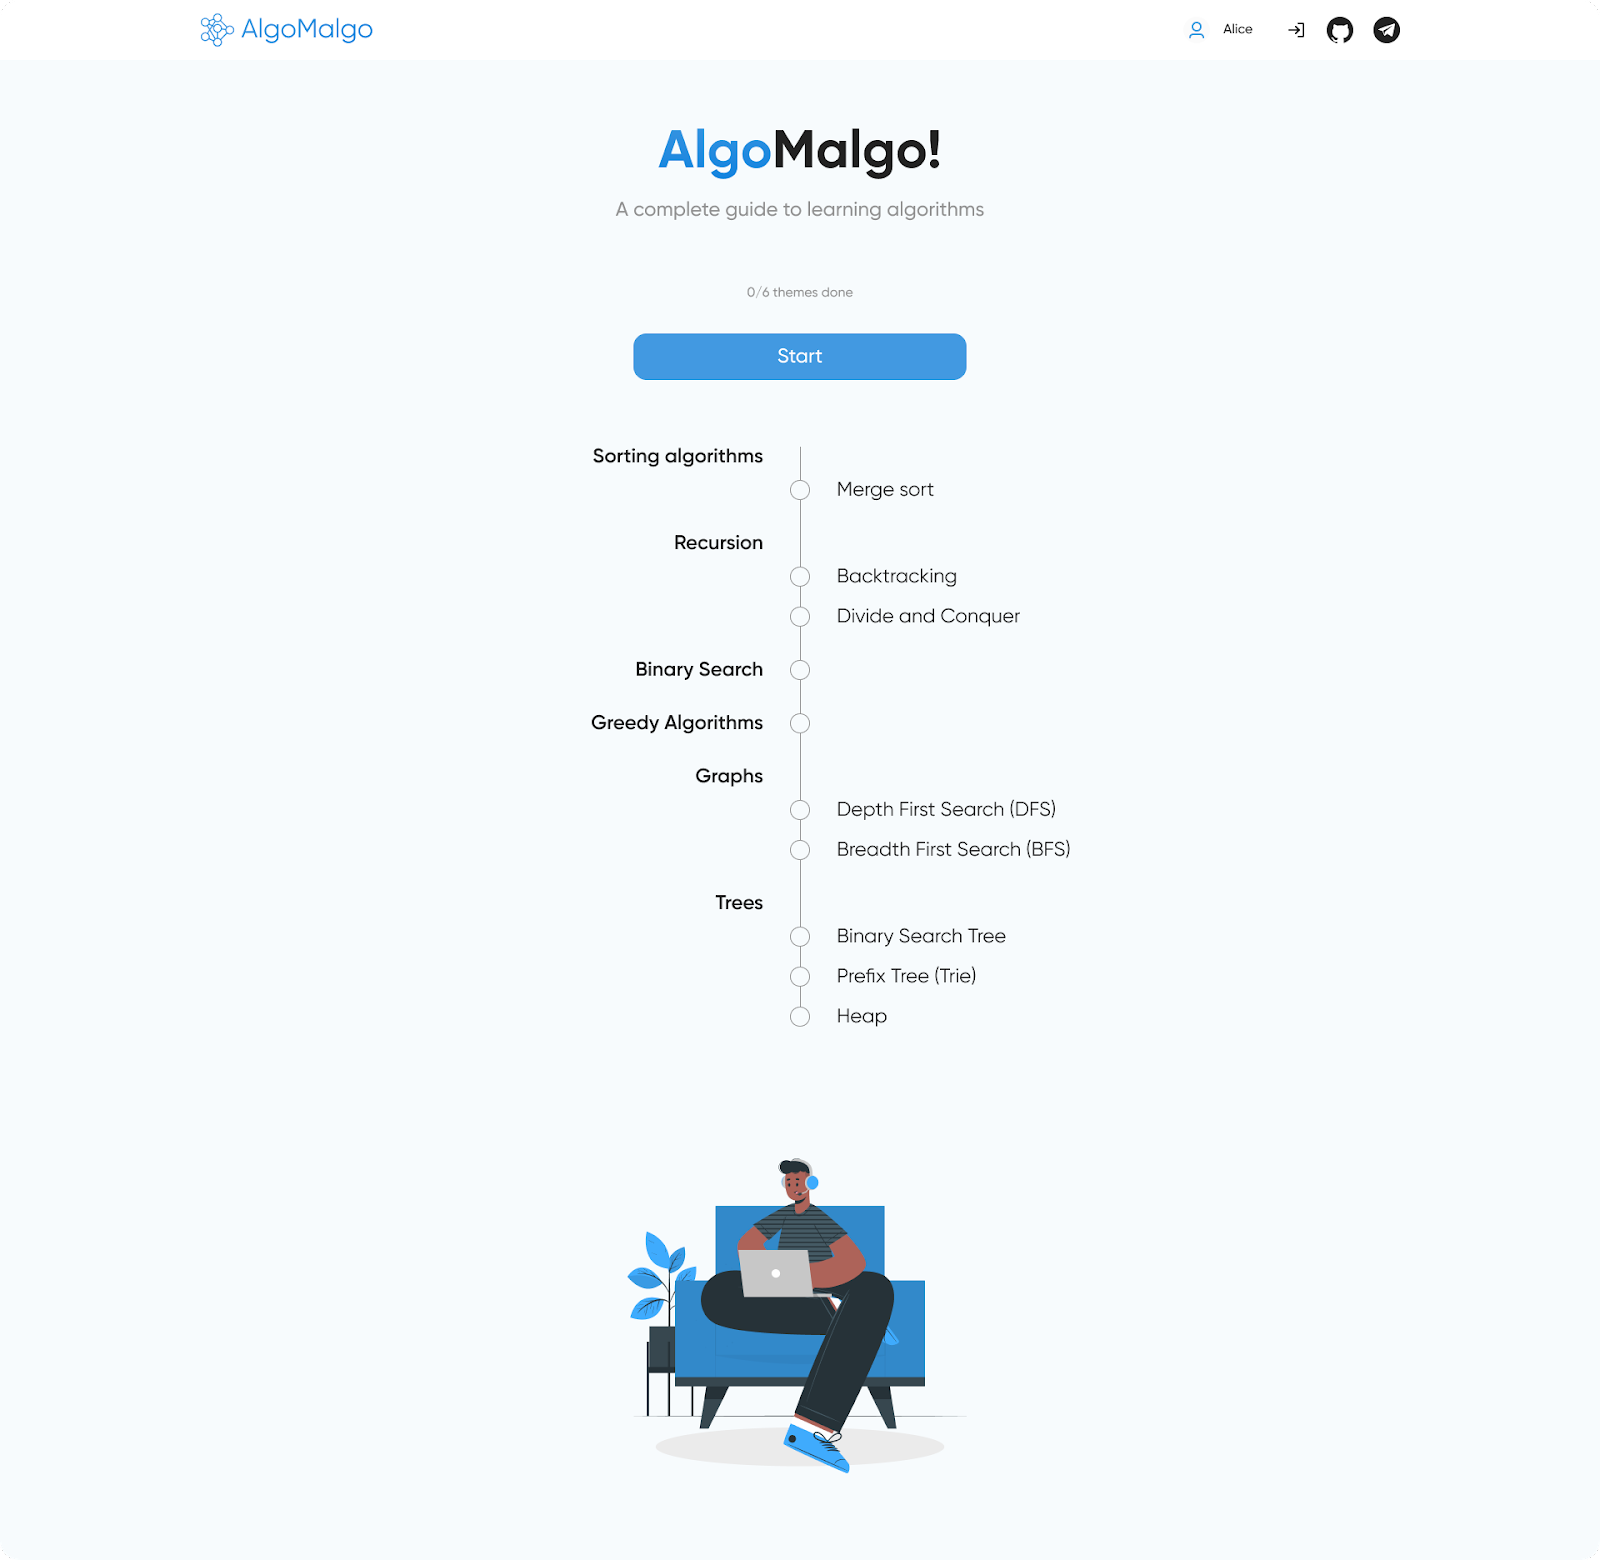
\includegraphics[scale=0.3]{figures/homepage.png}
    \caption{Home Page}
    \label{fig:gp}
\end{figure}


\pagebreak

\begin{figure}[h]
    \centering
    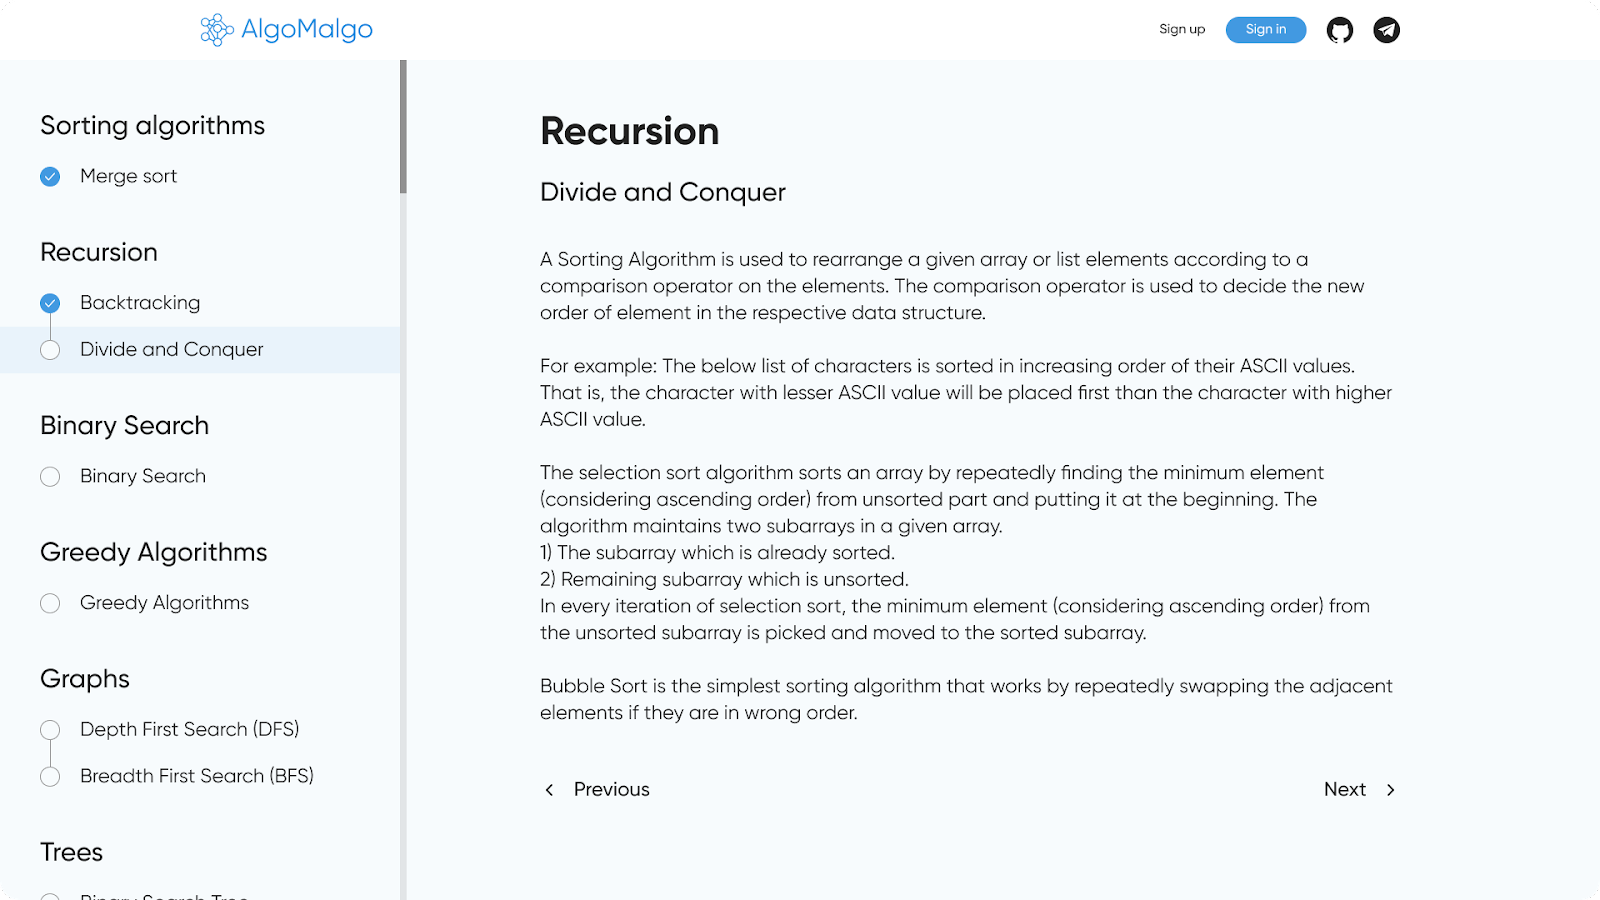
\includegraphics[scale=0.3]{figures/content.png}
    \caption{Content}
    \label{fig:gp}
\end{figure}


\pagebreak

\begin{figure}[h]
    \centering
    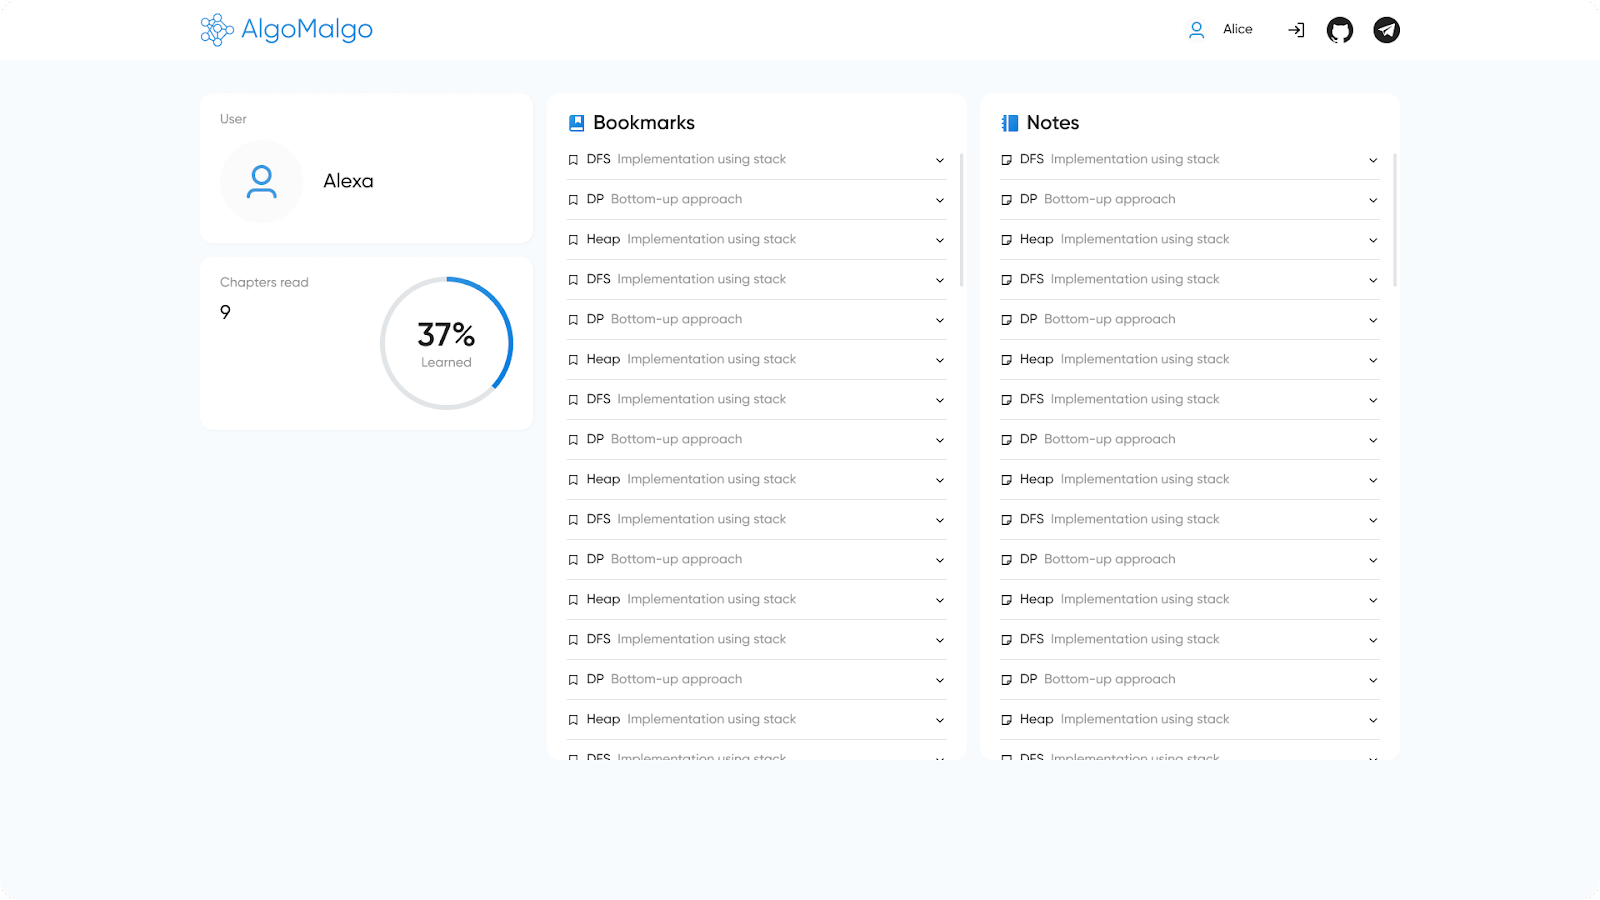
\includegraphics[scale=0.3]{figures/dashboard.png}
    \caption{Dashboard}
    \label{fig:gp}
\end{figure}


\pagebreak

\subsection{System Architecture}
System architecture of AlgoMalgo will be based on microservice, due its scalability and flexibility. Thus, with the increasing demand for our service, system design of website will change. As a main cloud computer provider AWS will be used, because of its cost-efficiency, flexibility and scalability.


\begin{figure}[h]
    \centering
    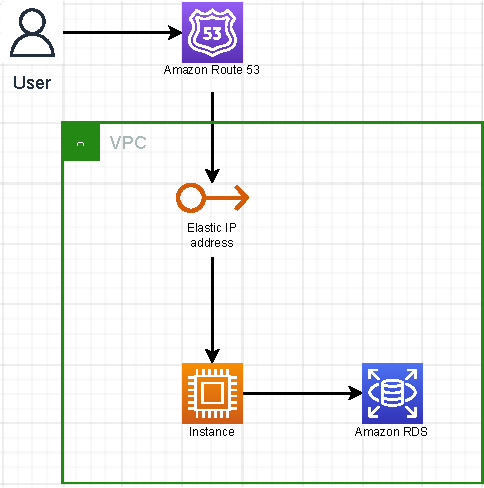
\includegraphics[scale=0.85]{figures/d1.pdf}
    \caption{100 users}
    \label{fig:gp}
\end{figure}


\pagebreak

In the above diagram, architecture is focused to embrace the number of users from 100 to 1000. As a main components Amazon Route 53, Elastic IP address, Instance and Amazon RDS will be used. All of them will be under virtual private cloud (VPC).

\begin{itemize}
  \item Amazon Route 53 component will be an extremely reliable and cost effective way to route end users to Internet applications by translating domain names to the ip address of our instances.
  \item Elastic IP address is used to mask the failure of an instance or software by instantly remapping the address to another instance in the user's AWS account.
  \item Instance is a server where app will be hosted
  \item Amazon RDS is a highly efficient solution for our relational database needs
\end{itemize}


\begin{figure}[h]
    \centering
    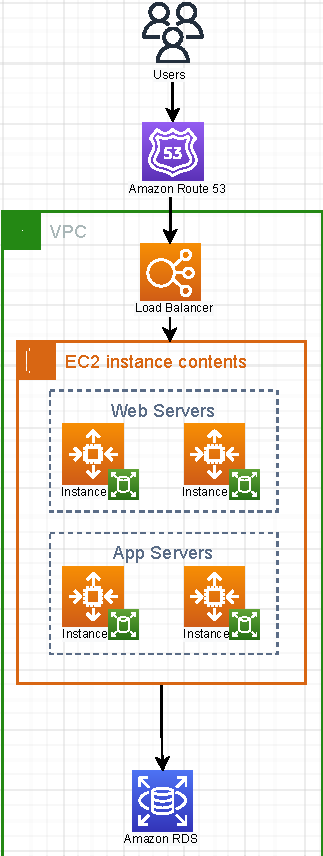
\includegraphics[scale=0.85]{figures/d2.pdf}
    \caption{1000 users}
    \label{fig:gp}
\end{figure}

\begin{itemize}
  \item EC2 instances will be used instead of simple instances, because of its auto-scaling capabilities. This feature will be helpful, in the situations, when the number of users will exceed the normal expectations. Thus, in days of extreme load, our application will remain healthy
  \item Elastic Block Stores is a green component attached to each EC2 instance in the above diagram. It serves as a cache block to each EC2 instance, so that service will remain fast.
  \item Load Balancer is a key component in every system that has more than 10000 users. This entity used to evenly distribute the load across existing EC2 instances to remain stability of the existing system.
\end{itemize}

To maintain the number of users from 1000 to 50000, Load Balancer, EC2 instances will be used. Furthemore, to evenly distribute the load, application logic and web logic will be hosted on different servers.

\begin{figure}[h]
    \centering
    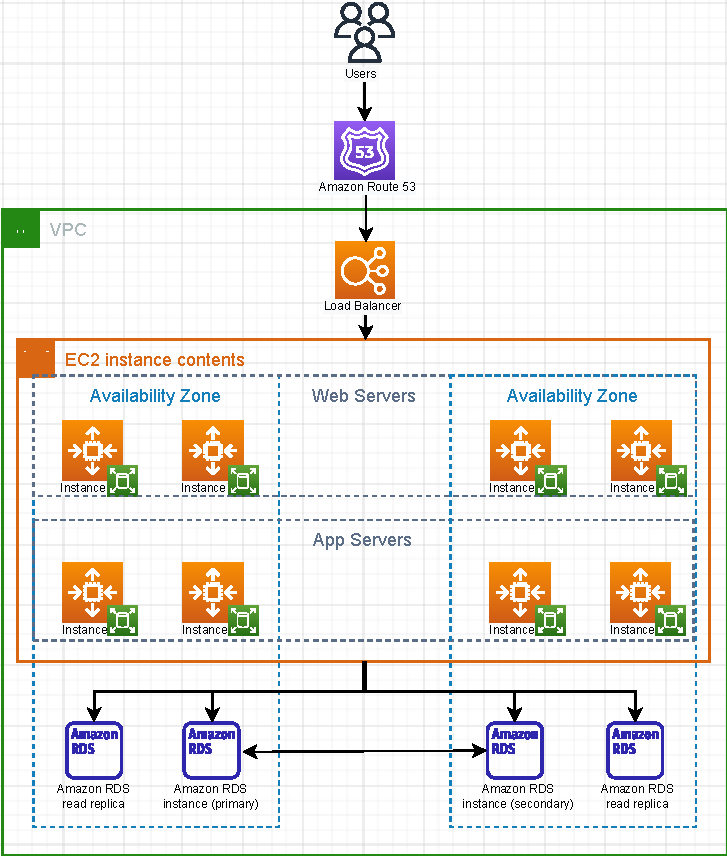
\includegraphics[scale=0.85]{figures/d3.pdf}
    \caption{1000 users}
    \label{fig:gp}
\end{figure}

Diagram above, indicates a good system architecture that could maintain the number of users from 50000 to 200000. Key components of the new system are RDS read replicas, RDS primary and secondary instances, and different availability zones.

\begin{itemize}
  \item RDS read replicas used to lower the load from RDS primary replicas, so that primary RDS replicas will handle only write requests. In the application it is supposed that the read operation requests will outperform by the number write requests. When the number of users will increase, the number of read replicas will increase proportionally.
  \item Availability Zone is a specific data point where EC2 instances and RDS components will be hosted. More Availability Zones indicate different data points, which will be located in different areas, so that users will not experience delays due their different locations across the country.
\end{itemize}


\begin{figure}[h]
    \centering
    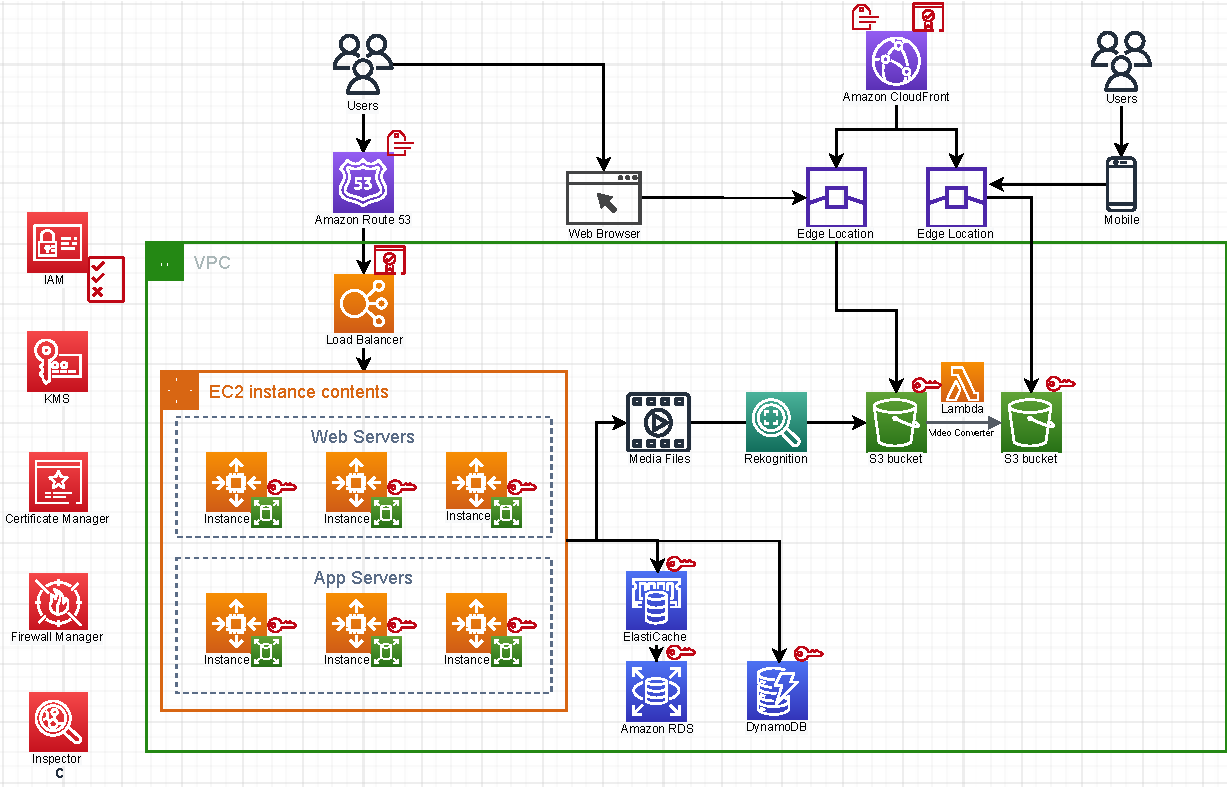
\includegraphics[scale=0.5]{figures/d4.pdf}
    \caption{10000 users}
    \label{fig:gp}
\end{figure}

System architecture shown above designed to support the number of users from 200000 to 1 million. There are many new components such as: IAM, KMS, Certificate Manager, Firewall Manager, Inspector, Rekognition, S3 buckets, Lambda, ElastiCache, DynamoDB, EdgeLocation and Amazon CloudFront. Services as IAM, KMS, Certificate Manager, Firewall Manager and Inspector responsible for security measures. They provide great security out of box, which will be essential for a service having around 1 million users. Different availability zones, Database read replicas not shown in this diagram to keep it clean. \\

\begin{itemize}
  \item Identity Access Manager is IAM in short. It is a primary service for managing all accesses of users in our AWS system. Accesses, authentication, authorization, restrictions managed by IAM. It will be used to give different permissions to a particular set of users, to manage an entire architecture.
  \item Key Management Service is KMS in short. It is a primary service responsible for all encryptions of data across the system. Services like DynamoDB, AmazonRDS, ElastiCache, S3 buckets and elastic block stores will be affected by KMS.
  \item Certificate Manager will be mainly responsible for providing SSL certificate to make secure HTTPS connections to services like Load balancer and Amazon CloudFront.
  \item Firewall Manager’s key responsibility is preventing different web site attacks including cross-site scripting, SQL injections, DDoS attacks, etc. This application firewall will secure such components as Amazon Route 53 and Amazon CloudFront.
  \item Inspector scans existing machines for the purpose of finding any known vulnerabilities, so that developers will fix them.
  \item Rekognition serves as a content filter, which will find out inappropriate objects in an image and will prevent this image being uploaded to S3 bucket.
  \item S3 bucket is an unlimited external storage, content on that storage could be accessible from any endpoint on the internet. In our system S3 bucket is mainly used for storing user media files, like images and videos.
  \item Lambda is a serverless service of Amazon, which will be used to convert one media format to another. It is expected that having 1 million users, that some of them will access AlgoMalgo through mobile phones. To maintain good user experience, it is essential to convert media files specifically for their devices.
  \item ElastiCache is a cache service for RDS databases. It comes with Redis and Memcached engines in it. Using ElastiCache we will reduce database calls, so that data that is accessed often will not heavily load RDS.
  \item DynamoDB is a NoSQL database solution. It will be essential for storing BookMarks and Notes logic. Currently, BookMarks and Notes stored in RDS, however having 1 million users it will be a wise decision to store these data on NoSQL database.
  \item Edge Location is a nearest location, where static content will be cached.
  \item CloudFront is a content delivery network (Cache), that is used for caching static content through accessing the nearest edge location. It is a good solution for caching any media content like images and videos. Because our system consists of detailed video explanations of algorithms and has various images explaining step by step solutions, it would be a great idea to have such service.
\end{itemize}
